%----------------------------------------------------------------------------
% \documentclass[letterpaper,10pt,twocolumn]{IEEEtran} 
% \documentclass[a4paper,10pt,conference]{ieeeconf} 
% \documentclass[conference,10pt,letterpaper,final]{IEEEtran}
% \documentclass[conference,letterpaper,final]{IEEEtran} % config for upload final
%----------------------------------------------------------------------------
\documentclass[conference]{IEEEtran}
\IEEEoverridecommandlockouts

%----------------------------------------------------------------------------
% CHOOSE language 
\usepackage[english]{babel} 
% => admissible choices for figure generation: {english},{} (standard, may be emtpy) or {german}
\def\chosenlanguage{english} 
%----------------------------------------------------------------------------

%----------------------------------------------------------------------------
% INCLUDE LMRES Preamble
\input{LMRES_PathDefinitions_Template} % define local path to LMRES Templates
\input{\LMRESTEMPLATESPATH/include_preambles/LMRES_Preamble}
%----------------------------------------------------------------------------

%----------------------------------------------------------------------------
% THIS IS NEEDED FOR FINAL SUBMISSION
%\IEEEoverridecommandlockouts 
% This command is only needed if you want to use the \thanks commands  
%\overrideIEEEmargins 
% Needed to meet printer requirements.
%---------------------------------------------------------------------------- 

%----------------------------------------------------------------------------
% DEFINE MORE INDIVIDUAL PATHS, e.g.
% \newcommand*{\PARTSPATH}{\LMRESTEMPLATESPATH/parts}
% \newcommand*{\FIGURESPATH}{./figures}
% \newcommand*{\MOVIESPATH}{./movies}
% ... add more if required
%----------------------------------------------------------------------------

%----------------------------------------------------------------------------
% INCLUDE MORE INDIVIDUAL PACKAGES, e.g.	
% LASTPAGE - find lastpage [does not work with TIKZ!]
% \usepackage{lastpage}
% IEEE trantools
% \usepackage{\IEEEPATH/IEEEtrantools}
% HYPERREF
\usepackage{hyperref}
\hypersetup{
	pdftoolbar=false,        	% show Acrobat’s toolbar?
	pdfmenubar=false,        	% show Acrobat’s menu?
	pdffitwindow=false,     	% window fit to page when opened
	pdfstartview={FitH},    	% fits the width of the page to the window
	pdftitle={},    	% title
	pdfauthor={},     	% author
	%     pdfsubject={},   	% subject of the document
	%     pdfcreator={},   	% creator of the document
	%     pdfproducer={}, 	% producer of the document
	%     pdfkeywords={keyword1, key2, key3}, % list of keywords
	%     pdfnewwindow=true,      	% links in new PDF window
	colorlinks=true,       	% false: boxed links; true: colored links
	linkcolor=blue,          	% color of internal links (change box color with linkbordercolor)
	citecolor=blue,       	% color of links to bibliography
	filecolor=blue,      	% color of file links
	urlcolor=blue		% color of external links
}
\usepackage{cleveref, autonum}
% ... add more if required
%----------------------------------------------------------------------------

%----------------------------------------------------------------------------
% INCLUDE MORE INDIVIDUAL MACROS, e.g.
\newtheorem{theorem}{Theorem}
\newtheorem{assum}{Assumption}
\newcommand{\MSRY}[1]{{\color{red} [MS: #1]}} % Myeongseok's comment
% ... add your own if required
%----------------------------------------------------------------------------

%----------------------------------------------------------------------------
% INCLUDE MORE INDIVIDUAL SYMBOLS, e.g.
% ... add your own if required
\newcommand\etal{\textit{et~al.\ }}
\newcommand\eg{\textit{e.g.\ }}
\newcommand\ie{\textrm{i.e.\ }}

% \newcommand\f{\mathbf{f}}
% \newcommand\bfB{\mathbf{B}}
%----------------------------------------------------------------------------

%----------------------------------------------------------------------------
% USE NEW NOTATION in dq (instead of k) and alphabeta (instead of s), phip (instead of phik) ... etc
\renewcommand*{\kCOSY}{dq}
\renewcommand*{\sCOSY}{\alpha\beta}
\renewcommand*{\rCOSY}{\alpha_{\ROTOR}\beta_{\ROTOR}}
% ... if you want to stick with old notation, remove lines above.
%----------------------------------------------------------------------------

%----------------------------------------------------------------------------
% *** Do not adjust lengths that control margins, column widths, etc. ***
% *** Do not use packages that alter fonts (such as pslatex).         ***
% There should be no need to do such things with IEEEtran.cls V1.6 and later.
% (Unless specifically asked to do so by the journal or conference you plan
% to submit to, of course. )

% correct bad hyphenation here
\hyphenation{op-tical net-works semi-conduc-tor}
\pagestyle{empty}
%----------------------------------------------------------------------------

%----------------------------------------------------------------------------
\begin{document}
% paper title
% % can use linebreaks \\ within to get better formatting as desired
\title{
    Constrained Optimization-Based Neuro-Adaptive Control (CoNAC) for Synchronous Machine Drives Under Nonlinear Voltage Saturation
% {\footnotesize \textsuperscript{*}Note: Sub-titles are not captured for https://ieeexplore.ieee.org  and
% should not be used}
    \thanks{
        This work was supported by GIST-IREF from Gwangju Institute of Science and Technology(GIST).
    }
}
%
%
% author names and IEEE memberships
% note positions of commas and nonbreaking spaces ( ~ ) LaTeX will not break
% a structure at a ~ so this keeps an author's name from being broken across
% two lines.
% use \thanks{} to gain access to the first footnote area
% a separate \thanks must be used for each paragraph as LaTeX2e's \thanks
% was not built to handle multiple paragraphs
%

\author{
    \IEEEauthorblockN{1\textsuperscript{st} Myeongseok Ryu}
    \IEEEauthorblockA{\textit{School of Mechanical and Robotics Engineering} \\
    \textit{Gwangju Institute of Science and Technology}\\
    Gwangju, Republic of Korea \\
    dding\_98@gm.gist.ac.kr}
\and
    \IEEEauthorblockN{2\textsuperscript{nd} Niklas Monzen}
    \IEEEauthorblockA{\textit{Laboratory for Mechatronic and Renewable Energy Systems (LMRES)} \\
    \textit{Hochschule München (HM) University of Applied Sciences}\\
    Munich, Germany \\
    niklas.monzen@hm.edu}
\and
    \IEEEauthorblockN{3\textsuperscript{rd} Christoph M Hackl}
    \IEEEauthorblockA{\textit{Laboratory for Mechatronic and Renewable Energy Systems (LMRES)} \\
    \textit{Hochschule München (HM) University of Applied Sciences}\\
    Munich, Germany \\
    christoph.hackl@hm.edu}
\and
    \IEEEauthorblockN{4\textsuperscript{th} Kyunghwan Choi}
    \IEEEauthorblockA{\textit{School of Mechanical and Robotics Engineering} \\
    \textit{Gwangju Institute of Science and Technology}\\
    Gwangju, Republic of Korea \\
    khchoi@gist.ac.kr}
}

% note the % following the last \IEEEmembership and also \thanks - 
% these prevent an unwanted space from occurring between the last author name
% and the end of the author line. i.e., if you had this:
% 
% \author{....lastname \thanks{...} \thanks{...} }
%                     ^------------^------------^----Do not want these spaces!
%
% a space would be appended to the last name and could cause every name on that
% line to be shifted left slightly. This is one of those "LaTeX things". For
% instance, "\textbf{A} \textbf{B}" will typeset as "A B" not "AB". To get
% "AB" then you have to do: "\textbf{A}\textbf{B}"
% \thanks is no different in this regard, so shield the last } of each \thanks
% that ends a line with a % and do not let a space in before the next \thanks.
% Spaces after \IEEEmembership other than the last one are OK (and needed) as
% you are supposed to have spaces between the names. For what it is worth,
% this is a minor point as most people would not even notice if the said evil
% space somehow managed to creep in.

% The paper headers
%\markboth{Mediterranean Conference on Control and Automation, June 20-23 2011}%,~Vol.~x, No.~x, xxx~2011}%
%{Shell \MakeLowercase{\textit{et al.}}: Bare Demo of IEEEtran.cls for Journals}
% The only time the second header will appear is for the odd numbered pages
% after the title page when using the twoside option.
% 
% *** Note that you probably will NOT want to include the author's ***
% *** name in the headers of peer review papers.                   ***
% You can use \ifCLASSOPTIONpeerreview for conditional compilation here if
% you desire.

% If you want to put a publisher's ID mark on the page you can do it like
% this:
%\IEEEpubid{0000--0000/00\$00.00~\copyright~2007 IEEE}
% Remember, if you use this you must call \IEEEpubidadjcol in the second
% column for its text to clear the IEEEpubid mark.

% use for special paper notices
%\IEEEspecialpapernotice{(Invited Paper)}


%----------------------------------------------------------------------------
% TITLE
\maketitle 
% set page style
\thispagestyle{empty}
%----------------------------------------------------------------------------

%----------------------------------------------------------------------------
% ABSTRACT
\begin{abstract}
	This paper demonstrates the effectiveness of the Constrained Optimization-Based Neuro-Adaptive Control (CoNAC) for synchronous machines.
	\color{blue}\lipsum[1]\color{black}
\end{abstract}
%----------------------------------------------------------------------------

% IEEEtran.cls defaults to using nonbold math in the Abstract.
% This preserves the distinction between vectors and scalars. However,
% if the journal you are submitting to favors bold math in the abstract,
% then you can use LaTeX's standard command \boldmath at the very start
% of the abstract to achieve this. Many IEEE journals frown on math
% in the abstract anyway.

% Note that keywords are not normally used for peerreview papers.
\begin{IEEEkeywords}
	Synchronous Machine Drives, Constrained Optimization, Neuro-Adaptive Control
\end{IEEEkeywords}

%----------------------------------------------------------------------------
% MAIN
% ============================================
%         SECTION: Introduction
% ============================================
\section{Introduction}

Synchronous machines are widely used in various industrial applications, such as ...

Due to the nonlinear nature of the synchronous machines (SMs), the control design for the SMs is challenging.
The representative nonlinear natures are the parameter (\eg inductance, ...) uncertainties and the voltage saturation.

Voltage source converters (VSCs)

For the parameter uncertainties, typically, first(?) and regular experimental implementation are conducted to identify a nominal values or look-up tables for the system parameters.

On the other hand, Adaptive methods ...
Neuro-adaptive control (NAC)
neural network (NN)
\MSRY{Literature review}

In author's previous work, the Constrained optimization-based neuro-adaptive control (CoNAC) was proposed for Euler-Lagrange systems with unknown system dynamics and constraints.

Motivated by above discussion, the main contributions of this paper are listed as follows:
\begin{itemize}
    \item The prior system parameters (\eg inductance, ...) is not required for control, since the NN in the CoNAC approximates the unknown system dynamics, including the system parameters.
    \item Voltage saturation is considered in the CoNAC as a corresponding control input constraint function. In other word, ...
    \item The boundedness of the tracking error and the NN weights are guaranteed by the Lyapunov stability analysis. ...
    \item The Karsh-Kuhn-Tucker (KKT) conditions are satisfied in steady state, which implies that the CoNAC is optimal in the sense of the constrained optimization, and demonstrated by numerical simulation(?).
\end{itemize}

\color{blue}\lipsum[1-4]\color{black}

% ============================================
%         SECTION: Problem Statement
% ============================================
\section{Problem Statement}

\subsection{Notations}

In this paper, following notations are used:
\begin{itemize}
    \item $\otimes$ denotes the Kronecker product {\cite[Definition 7.1.2]{Bernstein:2009aa}}.
    \item $x_{(i)}$ denotes the $i\textsuperscript{th}$ element of the vector 
    \item $\text{row}_i(A)$ denotes the $i\textsuperscript{th}$ row of the matrix $A\in\mathbb{R}^{n\times m}$. 
    \item $\text{vec}(A)\triangleq [\text{row}_1(A^T)  ,\cdots,\text{row}_m(A^T)  ]^T   $ for $A\in\mathbb{R}^{n\times m}$.
    \item $\lambda_\text{min}(A)$ denotes the minimum eigenvalue of the matrix $A\in\mathbb{R}^{n\times n}$.
\end{itemize}

\subsection{Synchronous Machine Dynamics and Control Objective}

Consider the SMs modeled by
\begin{equation}
	\usdq = \Rsdq \isdq + \omegaP \J \psisdq+ \ddt\psisdq
	\label{eq:model1}
\end{equation}
where $\J \triangleq \text{diag}([-1,+1])$, stator voltages $\usdq \triangleq [\usd, \usq]^T$, stator current $\isdq \triangleq [\isd, \isq]^T$, stator resistance matrix $\Rsdq \triangleq \Rsdq(\isdq, \phiP, \omegaP)\in \R^{2\times2}$, and electrical angular angle $\phiP$ and velocity $\omegaP$.
In general, the stator flux linkages $\psidq \triangleq \psidq(\isdq, \phiM)$, depend on currents $\isdq$ and mechanical angle $\phiM$ which is $\omegaP$ divided by pole pair number $nP$.
Therefore, the last term of \eqref{eq:model1} can be written as $\ddt \psisdq = [{\DERIVATIVE\over \DERIVATIVE\isdq}\psisdq] \ddt \isdq + [{\DERIVATIVE\over \DERIVATIVE\phiM}\psisdq] \ddt \phiM$, where ${\DERIVATIVE\over \DERIVATIVE\isdq}\psisdq$ is typically referred to differential inductance matrix $\Lsdq\triangleq\Lsdq(\isdq, \phiM)$.
This allows to rewrite \eqref{eq:model1} as current dynamics as follows:
\begin{equation}
	\ddt \isdq = (\Lsdq)^{-1}(\usdq - \Rsdq \isdq - \omegaP \J \psisdq)
	\label{eq:model2}
	.
\end{equation}
Assuming that the electrical angular speed (and position) is constant, $\Rsdq,\psisdq$ and $\Lsdq$ are only depends on the stator currents $\isdq$.

For convenience, \eqref{eq:model2} is rewritten in the standard control-affine form as follows:
\begin{equation}
	\dot x = f(x) + B(x) u
	\label{eq:model3}
\end{equation}
where state variable $x \triangleq \isdq\in\R^2$, control input variable $u \triangleq \usdq\in\R^2$, system function $f(x) \triangleq -(\Lsdq)^{-1}(\Rsdq \isdq + \omegaP \J \psisdq):\R^2\to\R^2$, and input matrix $B(x) \triangleq (\Lsdq)^{-1}:\R^2\to\R^{2\times 2}$.

It is notable that $f(x)$ and $B(x)$ are continuous bounded nonlinear functions such that $\Vert f(x)\Vert \le \bar f<\infty$ and $\Vert B(x)\Vert \le \bar g<\infty$, respectively
In addition, since inductance matrix $\Lsdq$ is positive definite matrix, $B(x)$ is positive definite matrix implying that a matrix $(1/2)(B(x)+B(x)^T)$ is uniformly positive definite for all $x\in\Omega_x$ where $\Omega_x\subset\R^2$ is a compact set and there exists a positive lower bound constant $\underbar{b}\in\R_{>0}$ of the smallest singular value such that $\lambda_\text{min} [(1/2)(B(x)+B(x)^T)] \ge \underbar b >0,\ \forall x\in\Omega_x$.
This guarantees that the system \eqref{eq:model3} is uniformly controllable \cite{Xu:2003aa} \MSRY{Find better ref}.

Due to the voltage saturation of the VSCs, the control input $u$ is constrained as follows:
\begin{equation}
	u \leftarrow {u\over \Vert u\Vert} \bar u
\end{equation}
where $\bar u\triangleq \umax$ is the maximum voltage amplitude of the VSCs.

The objective of this paper is to design a neuro-adaptive control that enables $\isdq$ track a feasible continuously differential reference signal $x_d \triangleq \isdqref(t):\R\to\R^2$ for the SMs under the voltage saturation.

% ============================================
%        SECTION: Controller Design
% ============================================
\section{Controller Design}

\subsection{Neuro-Adaptive Control Design}

As discussted in \cite{Xu:2003aa}, 
Motivated by feedback-linearzation control method, a stabilizing control input $u^*$ can be designed as follows:
\begin{eqnarray}
	u^* = B^{-1}(x) [ -f(x) +Ae + \dot x_d]
	\label{eq:ideal_control}
\end{eqnarray}
where $e\triangleq x-xd$ denotes the tracking error of stator current, and $A\in\R^{2\times 2}$ is a Hurwitz matrix. 
Using \eqref{eq:model2} and \eqref{eq:ideal_control}, one can obtain the following error dynamics:
\begin{equation}
	\dot e = Ae + B(x) 
	[
		u-u^*
	]
	.
	\label{eq:error_dynamics1}
\end{equation} 
However, since the system dynamics are unknown, $u^*$ cannot be realized in practice.
Inspired by \cite{Hart:2023aa} and [...], the CoNAC proposed in \cite{Ryu:2024aa} is modified for the SMs.

Since the motor controller should have high sample rate, the NN in CoNAC is simplified to one hidden layer NN which is represented as
\begin{equation}
	\Phi(x_n;\theta) = V_1^T\phi(V_0^Tx_n)
	\label{eq:NN}
\end{equation}
where $V_i\in\R^{(l_i+1)\times l_{i+1}},\ \forall i\in[0,1]$ is the weight matrix, $\phi:\R^{l_{1}} \to \R^{l_{1}+1}$ is the activation function, and $x_n\in\R^{l_0}$ is the input vector.
For simplicity, the weight matrices are augmented as $\theta\triangleq[\theta_0^T, \theta_1^T]^T\in\R^{\Xi}$, where $\theta_i\triangleq \text{vec}(V_i)\in\R^{\Xi_i}$.
The activation function is defined as element-wise nonlinear function $\sigma(\cdot):\R\to\R$ and augmentation $1$ to account for bias term in the weight matrices such that $\phi(x) = [\sigma(x_{(1)}),\cdots,\sigma(x_{(l_1)}),1]^T$.
The nonlinear function $\sigma(\cdot)$ is chosen as $\tanh(\cdot)$ in this paper for the boundedness of its output and gradient.

According to the universal approximation theorem \cite{Cybenko:1989aa,Barron:1993aa}, NNs whose activation functions are sigmoidal functions (\eg sigmoid or $\tanh(\cdot)$) can approximate any continuous nonlinear function (\ie $u^*$) with $\epsilon$-accuracy in a compact set $x_n\in\Omega$ such that $\sup_{x_n\in\Omega} \Vert \Phi(x_n;\theta^*) - u^*\Vert = \epsilon<\infty$ for some positive constant $\epsilon\in\R_{>0}$, where $\theta^*\in\R^\Xi$ denotes the ideal weight vector.
Since the ideal weight vector is unknown, the ideal weight vector is estimated as $\hat\theta_k\in\R^\Xi$ and used in controller.

Substituting ideal and estimate weights in \eqref{eq:error_dynamics1}, the following error dynamics can be obtained:
\begin{equation}
	\dot e = Ae + B(x) 
	[
		\hat\Phi - \Phi^* -\epsilon	
	] 
	\label{eq:error_dynamics2}
\end{equation}
where $\hat\Phi\triangleq \Phi(x;\hat\theta_k)$ and $\Phi^*\triangleq \Phi(x;\theta^*)$.
According to \eqref{eq:error_dynamics2}, the tracking error $e$ can be driven to zero by adapting the estimate weight vector $\hat\theta_k$ such that $\Phi(x;\hat\theta_k) \to \Phi(x;\theta^*)$, assuming $\epsilon$ is sufficiently small.

\subsection{Constrained Optimization-Based Adaptation Law Derivation}

The adaptation law of CoNAC is derived by the constrained optimization theory.
First, the control problem is represented as the following optimization problem:
\begin{equation}
	\begin{matrix}
		\min_{\hat\theta\in\Omega}
		J(e;\hat\theta)={1\over2} e^Te 
		,\\ \\
		\text{subject to }\ 
		\begin{cases}
			c_{\theta_i(\hat\theta)}= 
			\hat\theta_i^T\hat\theta_i-\bar\theta_i^2 \le 0,
			&\forall i\in[0,1]
			\\
			c_u(\hat\theta) 
			=\hat\Phi^T\hat\Phi  - \bar u^2  \le 0
		\end{cases}
	\end{matrix}
		\label{eq:opt_problem}
\end{equation}
where $J:\R^2\times\R^2\to\R$ is the positive definite objective function, $c_{\theta_i}:\R^{\Xi_i}\times\R^{\Xi_i}\to \R$ and $c_u:\R^2\times\R^2\to\R$ are the inequality constraint functions, and $\bar\theta_i\in\R_{>0}$ and $\bar u\in\R_{>0}$ are the positive maximum values of $\Vert\theta_i\Vert$ and $\Vert u\Vert$, respectively.
Here, the tracking error $e$ is considered as pre-defined data and the estimate weight vector $\hat\theta$ is the optimization variable.
The corresponding Lagrangian function of \eqref{eq:opt_problem} is defined as follows:
\MSRY{Do you prefer to use small summation and fractions?}
\begin{equation}
	L(e,\hat\theta,[\lambda_j]_{j\in\mathcal I}) 
	\triangleq
	J + \sum_{j\in\mathcal I} \lambda_j c_j
	\label{eq:lagrangian}
\end{equation}
where $\mathcal I\triangleq\{0,1,u\}$ is a set of imposed inequality constraint functions and $\lambda_j\in\R_{\ge0}$ are the Lagrange multipliers.

To solve the dual problem of \eqref{eq:opt_problem} (\ie $\min_{\hat\theta} \max_{\lambda_j\in\mathcal I} \allowbreak  L(e,\hat\theta,[\lambda_j]_{j\in\mathcal I})$), the adaptation law is derived as follows:
\begin{subequations}
	\begin{align}
		\dot {\hat\theta}&=-\alpha 
		\tfrac{\partial}{\partial \hat\theta} L
		=-\alpha 
		\bigg(
		{\partial J\over \partial \hat\theta}+\sum_{j\in\mathcal{I}}\lambda_j {\partial c_j\over\partial \hat\theta}
	\label{eq:adap_law:weight}
		\bigg)\\
		\dot\lambda_j& = \beta_j{\partial L\over\partial \lambda_j} = \beta_j c_j 
	\label{eq:adap_law:multiplier}
	\end{align}
	\label{eq:adap_law}
\end{subequations}
where $\alpha\in\R_{>0}$ and $\beta_j\in\R_{>0}$ are the adaptation gain and update rate of corresponding Lagrange multipliers, respectively.

In the adaptation law \eqref{eq:adap_law:weight}, one need to calculate the partial derivative of error with respect to the estimate weight vector $\partial e/\partial \hat\theta$ for $\partial J/\partial \hat\theta = (\partial e/\partial \hat\theta)^T e$.
In \cite{Ryu:2024aa}, the forward sensitivity method \cite{Sengupta:2014aa} is employed to obtain the sensitivity equation as follows:
\begin{equation}
	\ddt
	(
		% {\partial e\over\partial \hat\theta}
		\tfrac{\partial}{\partial \hat\theta} e
	)
	= 
	A
	\tfrac{\partial}{\partial \hat\theta} e
	+
	B(x)
	\tfrac{\partial}{\partial \hat\theta} \hat\Phi
	.
	\label{eq:sensitivity_eqn}
\end{equation}
Note that the initial value of $\partial e/\partial \hat\theta$ is zero matrix, since initial tracking error $e$ is independent on $\hat\theta$.
However, if the input matrix $B(x)$ is unknown, the sensitivity equation \eqref{eq:sensitivity_eqn} cannot be simulated.
Furthermore, simulating the sensitivity equation requires large memory allocation and computational cost, since in general the number of weights are large for NNs.

Therefore, 


% ============================================
%        SECTION: Stability Analysis
% ============================================
\section{Stability Analysis}    

\begin{theorem}
    For the dynamical system in \eqref{eq:model3}, the neuro-adaptive controller \eqref{eq:NN}, and weight adaptation law \eqref{eq:adap_law:weight} and \eqref{eq:adap_law:multiplier} ensure the boundedness of the tracking error $e$ and the weight estimate $\hat \theta$. 
	This holds with the weight norm constraint, provided that the control gains satisfy.
\end{theorem}

\begin{proof}

Consider the following Lyapunov function candidate:
\begin{equation}
	\mathcal V \triangleq {1\over 2} e^TPe + {1\over 2\alpha} \hat\theta^T\hat\theta
\end{equation}

Taking time-derivative of $\mathcal V$ yields:
\begin{equation}
	\begin{aligned}
		\dot {\mathcal V}
		=&
		e^T(A^TP+PA)e + e^TB(x)
		\bigg(
		\hat\Phi - \Phi^*-\epsilon
		\bigg)
		\\
		&
		-\hat\theta_k^T
		\bigg(
		{\partial \hat\Phi\over\partial \hat\theta_k}^T \Gamma^T e +
		\lambda_{\theta_k} \hat\theta_k
		+\lambda_u{\partial\hat\Phi\over\partial \hat\theta_k}^T \hat\Phi
		\bigg)
		\\
		=&
		e^TQe + e^T
		\bigg(
		B(x) 
		\underbrace{
		\hat V_k^T \hat\phi_k
		}_{= (I\otimes \hat\phi_k^T) \hat\theta_k}
		\bigg)
		+e^T
		B(x)
		(
		-V^{*T}_k \phi^*_k
		+\epsilon
		)
		\\
		&
		-\hat\theta_k^T
		(I\otimes\hat\phi_k^T)
		^T \Gamma^T e 
		-
		\lambda_{\theta_k} 
		\hat\theta_k^T\hat\theta_k
		%\\&
		-
		\lambda_u
		\underbrace{
		\hat\theta_k^T
		(I\otimes\hat\phi_k^T)^T
		}_{=\hat\Phi^T}
		 \hat\Phi
		\\
		=&
		e^TQe + e^T
		\underbrace{
		(B(x)-\alpha \Gamma)
		}_{\triangleq 2 \mathcal G}
		 (I\otimes \hat\phi_k^T)\hat\theta_k
		\\
		&
		-
		\lambda_{\theta_k}
		\hat\theta_k^T\hat\theta_k 
		\underbrace{
		-\lambda_u
		\hat\Phi^T\hat\Phi
		}_{<0}
		+e^T
		\underbrace{
		B(x)
		(
		-V^{*T}_k \phi^*_k
		+\epsilon
		)
		}_{\triangleq \Delta(\theta^*, x)}
		\\
		\le 
		& 
		\begin{bmatrix}
		e\\ \hat\theta
		\end{bmatrix}^T
		\underbrace{
		\begin{bmatrix}
		Q & \mathcal G\dfrac{\partial \hat\Phi}{\partial \hat\theta}
		\\
		\dfrac{\partial \hat\Phi}{\partial \hat\theta}^T\mathcal G^T
		& -\lambda_{\theta_k} I
		\end{bmatrix}
		}_{\triangleq \mathcal A}
		\begin{bmatrix}
			e\\ \hat\theta
		\end{bmatrix}
		+
		\begin{bmatrix}
			\Delta & 0
		\end{bmatrix}
		\begin{bmatrix}
			e\\ \hat\theta
		\end{bmatrix}
	\end{aligned}
\end{equation}

\end{proof}

% ============================================
%       SECTION: Simulation Validation
% ============================================
\section{Simulation Validation}

\subsection{Simulation Setup}

\begin{figure}[!t]
	\centering
	\includegraphics[width=0.99\linewidth]{
		src/simulink_simulation/figures/compare/Fig6.eps
		}
	\caption{
		The stator flux linkages of the synchronous machine at $\omega_p=0$.
		\MSRY{$\omega_p=0$ ??}
	}
	\label{fig:model_param}
\end{figure}

\subsection{Simulation Results}

\begin{figure}[!t]
    \centering
        \subfloat[
			Tracking result of $d$-axis stator current $\isd$.
		]{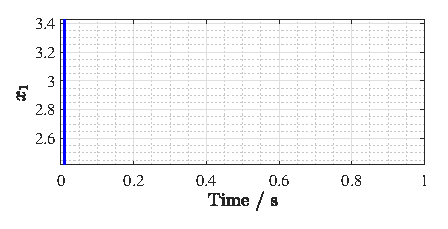
\includegraphics[width=0.99\linewidth]{
			src/simulink_simulation/figures/compare/Fig1.eps
			}%
        \label{fig:tracking_d}}
	\vspace{1mm}
		\subfloat[
			Tracking result of $q$-axis stator current $\isq$.
		]{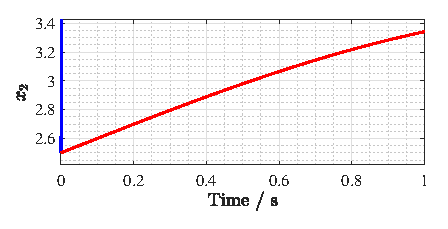
\includegraphics[width=0.99\linewidth]{
			src/simulink_simulation/figures/compare/Fig2.eps
			}%
        \label{fig:tracking_q}}
	\vspace{1mm}
		\subfloat[
			Norm of control input (stator voltages) $\usdq$.
		]{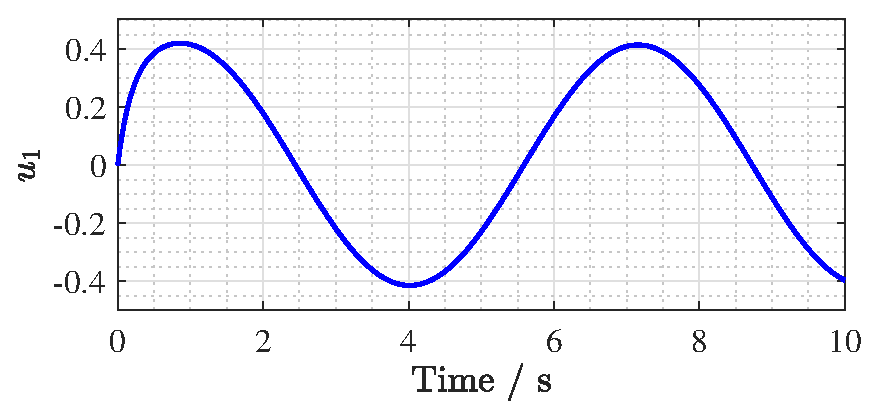
\includegraphics[width=0.99\linewidth]{
			src/simulink_simulation/figures/compare/Fig3.eps
			}%
        \label{fig:ctrl_norm}}
    \caption{
		Simulation results of the CoNAC with control input constraint $c_u$ (blue solid line) and without control input constraint (gray solid line), and reference signal of $\isdq$ (red dashed line) and maximum value of control input norm $\bar u$ (black solid line). 
	}
	
	\label{fig:ctrl_result1}
\end{figure}

\begin{figure}[!t]
    \centering
		\subfloat[
			Norm of weights $\hat\theta_i$.
		]{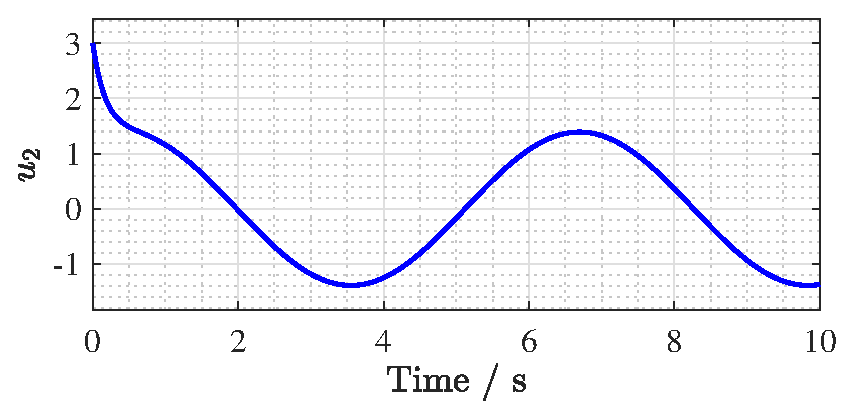
\includegraphics[width=0.99\linewidth]{
			src/simulink_simulation/figures/compare/Fig4.eps
			}%
        \label{fig:weights_norm}}
	\vspace{1mm}
		\subfloat[
			Lagrange multipliers $\lambda_j$ in logarithmic scale.
		]{\includegraphics[width=0.99\linewidth]{
			src/simulink_simulation/figures/compare/Fig5.eps
			}%
        \label{fig:multipliers}}
    \caption{
		Weight norms (a) of CoNAC with control input constraint $c_u$ (solid line) and without control input constraint (dash dotted line), and Lagrange multipliers (b) of the CoNAC with control input constraint $c_u$.
	}
	\label{fig:ctrl_result2}
\end{figure}

% ============================================
%            SECTION: Conclusion
% ============================================
\section{Conclusion}

%----------------------------------------------------------------------------

%----------------------------------------------------------------------------
% BIBLIOGRAPHY
\bibliographystyle{ieeetr}
% \bibliography{\BIBSPATH/LMRES_Bibliography}
\bibliography{refs}
%----------------------------------------------------------------------------

% that's all folks
\end{document}
%----------------------------------------------------------------------------

